\newpage
\subsection{Importing and working with multiple EAPs}
\visHeader
\label{sec:multiEAP}

\update with the Part6Visual download folder (desktop).

It should be mentioned here that the following instructions are about how to properly export and import EA files. You may want to bookmark this section so that
you can reference it later for your own projects.

\begin{itemize}

\item[$\blacktriangleright$] In the same \texttt{Part4.zip} folder you extracted this Part from, there's a \texttt{.eap} file called \texttt{FilesToImport}.
Double click this to open it in Enterprise Architect (EA).

\item[$\blacktriangleright$] Although you can simply copy and paste single packages between multiple EAPs, packages with dependencies to other packages (i.e.,
those between \texttt{DictionaryCodeAdapter} and \texttt{DictionaryLanguage}) cannot be copied so easily. If you do this, all links will be destroyed!
Therefore, to migrate multiple packages, you have to first export a \emph{complete} root node (the package on the top-most level of the project browser) to an
XMI file.

(1) Right click on root LearningBox2Dictioanry . Go to Import/Export, Export package as xmi file

(2) Save the file somewhere easily accessible, such as your desktop, and change the export type to \texttt{XMI 2.1}. the window won't close, but You should have
a small green bar appear once the action is complete (Fig.~\ref{fig:exportDialogue}).


\vspace{0.5cm}

\begin{figure}[htbp]
\begin{center}
  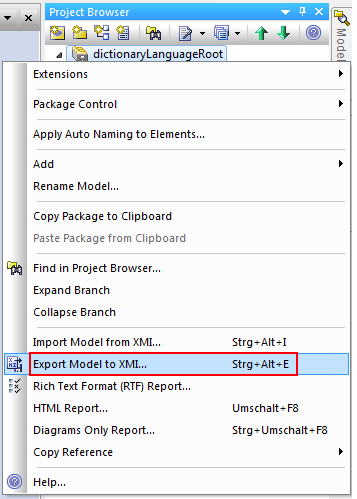
\includegraphics[width=0.5\textwidth]{ea_exportToXMI}
  \caption{Exporting the \emph{target metamodel}}
  \label{fig:export}
\end{center}
\end{figure}

% 
% \item[$\blacktriangleright$] Save the file somewhere easily accessible, such as your desktop, and change the export type to \texttt{XMI 2.1}. You should have a
% small green bar appear once the action is complete (Fig.~\ref{fig:exportDialogue}).

\vspace{0.5cm}

\begin{figure}[htbp]
\begin{center}
  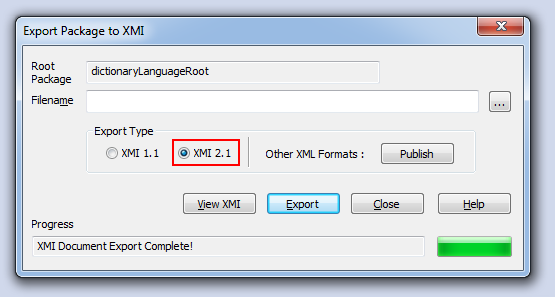
\includegraphics[width=0.8\textwidth]{ea_exportPackageDialogue}
  \caption{Persisting the export to a file}
  \label{fig:exportDialogue}
\end{center}
\end{figure}

\item[$\blacktriangleright$] Now open your \texttt{LeitnersLearningBox.eap} file, and right-click anywhere in the project browser
\texttt{Import Model from XMI\ldots}. 

\end{itemize}

In the dialogue that appears, find the file you just saved and \texttt{import}. Press \texttt{yes} in each of the confirmation dialogues
that appear after. Your workspace should now resemble Fig.~\ref{fig:postImport}.

(6) open and explore. In dictionary, you should be able to see stuff like dictionary, entry, etc etc..

() The new structure is automatically saved, so you dont have to worry about closing

(7) validate all and refersh your eclipse workspace. Dictionary adapter and language should appear under 'other projects' (generated code)
